%% Water Quality Prediction — Phase 2 Deep Learning Report
%% IEEE conference format; compile from this directory with pdfLaTeX or Tectonic.
\documentclass[conference]{IEEEtran}
\IEEEoverridecommandlockouts
\usepackage{cite}
\usepackage{amsmath,amssymb}
\usepackage{graphicx}
\usepackage{booktabs}
\usepackage{url}
\usepackage[hidelinks]{hyperref}
\graphicspath{{../../reports/figures/}}

\begin{document}
\title{Deep Learning for CCME Water Quality Index Estimation: Input Conditioning, Regularization, and a Leakage-Safe Hybrid Design}
\author{
\IEEEauthorblockN{Shaik Tajuddin}\IEEEauthorblockA{\textit{2401010436} \\ shaik.tajuddin2024@nst.rishihood.edu.in}
\and\IEEEauthorblockN{Parthraj Singh Bhati}\IEEEauthorblockA{\textit{2401010320} \\ parthraj.bhati2024@nst.rishihood.edu.in}
\and\IEEEauthorblockN{Himanshu Pandey}\IEEEauthorblockA{\textit{2401020095} \\ himanshu.h2024@nst.rishihood.edu.in}
\and\IEEEauthorblockN{Jivit Rana}\IEEEauthorblockA{\textit{2401010202} \\ jivit.rana2024@nst.rishihood.edu.in}
\and\IEEEauthorblockN{Satya Yadav}\IEEEauthorblockA{\textit{2401010427} \\ satya.yadav2024@nst.rishihood.edu.in}
}
\maketitle
\begin{abstract}
Phase 1 established a leakage-aware machine-learning pipeline for estimating the Canadian Council of Ministers of the Environment (CCME) Water Quality Index (WQI), comparing tree ensembles across full and partial measurement settings. Its results showed that high full-input accuracy largely reflects reconstruction of the index formula and that errors rise when contributing measurements are unavailable. Phase 2 extends this work with a configurable multilayer perceptron (MLP), while preserving the saved split and fitting preprocessing on training data only. A three-seed input-transformation study finds quantile-normal preprocessing gives validation mean absolute error (MAE) $0.8015\pm0.1002$. A five-seed architecture study reports a tuned MLP test MAE of 0.5344 at a 200,000-row training scale, while a separate five-seed regularization sweep finds no regularizer whose gain exceeds seed variation. A five-seed validation ablation reports that the residual hybrid improves root mean squared error (RMSE) over its XGBoost base and outperforms a plain average. A later controlled five-seed test comparison at 20,000 training rows confirms lower hybrid RMSE than its raw-feature XGBoost base, while engineered-feature XGBoost performs best overall. Calibration code is available, but no empirical calibration output is saved.
\end{abstract}
\begin{IEEEkeywords}water quality index, deep learning, multilayer perceptron, tabular regression, residual learning\end{IEEEkeywords}

\section{Introduction}
Water-quality monitoring programmes often need to estimate an interpretable index from incomplete measurements. The project uses the Canadian Council of Ministers of the Environment (CCME) WQI and treats its continuous value as a regression target. Phase 1 cleaned and documented the harmonized data, removed exact duplicate rows, retained anomaly and upstream-imputation indicators for analysis, created a persisted station-grouped train/validation/test split, and built shared preprocessing and evaluation interfaces. It established a median baseline and compared Random Forest and XGBoost, including engineered-feature ablations, bootstrap uncertainty, feature attribution, and a partial-measurement ladder.

Phase 1's central finding was that the eight chemical measurements are inputs to the published index formula. XGBoost's very high 8/8 score therefore measures near-formula reconstruction, not independent environmental prediction. The partial-measurement experiments showed performance degradation as formula inputs were withheld, making incomplete-measurement estimation a more meaningful use case. The full-input result remains useful as a reproducible benchmark, but it must be interpreted separately from genuine estimation.

This provided the reason to move to Phase 2: test a deep-learning model under the same leakage controls, determine how neural input conditioning and regularization affect performance, and assess whether a residual hybrid adds value beyond tree models. Tree ensembles remain strong tabular baselines, while neural networks are sensitive to feature scale, skew and regularization~\cite{grinsztajn2022why,gorishniy2021revisiting,kadra2021well}. Phase 2 preserves the saved split and adds neural input, architecture, regularization, residual-hybrid, and controlled five-seed comparisons. The companion IEEE-format report supplies Phase 1 context~\cite{phase2companion}; Phase 2 claims in this report use the current repository CSVs and notebooks. The hybrid uses area-grouped out-of-fold predictions to avoid same-site leakage.

\section{Background and Related Work}
\subsection{Tabular neural networks}
Benchmark studies find that gradient-boosted trees often remain competitive on medium-scale tabular data. They handle heterogeneous feature scales, irrelevant covariates and threshold-like structure with less preprocessing, while neural models can become competitive when their feature transformations and optimization are well chosen~\cite{grinsztajn2022why,shwartzziv2022tabular,borisov2022deep,gorishniy2021revisiting}. Specialized attention architectures such as TabNet provide a feature-selection mechanism, but a simple MLP remains a useful controlled baseline~\cite{arik2021tabnet}. The universal approximation result establishes representational capacity under its assumptions; it does not guarantee good generalization or practical optimization~\cite{hornik1989multilayer}.

\subsection{Regularization and hybrid learning}
Weight decay, dropout, batch normalization and early stopping act through different mechanisms and should be measured rather than stacked by default. Tabular neural-network benchmarks motivate searching regularization combinations, while dropout and AdamW provide distinct stochastic and parameter-shrinkage mechanisms~\cite{kadra2021well,srivastava2014dropout,ioffe2015batch,loshchilov2018decoupled}. Monte Carlo dropout has been proposed as an approximate Bayesian uncertainty method; neural calibration work motivates checking whether nominal confidence or interval coverage matches observed outcomes~\cite{gal2016dropout,guo2017calibration}. These references motivate the Phase 2 experiments, but do not substitute for measured calibration on this dataset. The experiment artifacts and their results are described in Sections~\ref{sec:results} and~\ref{sec:limitations}.

\section{Data and Evaluation Protocol}
The project uses the harmonized surface-water dataset described in Phase 1: 2,818,006 records after exact duplicate removal, five countries, 61,689 monitoring sites, eight measurements, and a continuous CCME index target. The target is bounded at 100 and has a point mass at that ceiling. The records also contain an upstream median-imputation signature; original missing values cannot be recovered reliably from the published table. These properties constrain interpretation of all scores.

The saved Phase 1 split groups by monitoring area so a site does not occur in multiple partitions. Phase 2 loads these persisted splits rather than regenerating them. Numeric preprocessing and categorical encoding are fitted using training data only. Country and waterbody type are one-hot encoded for the MLP; area is reserved for split grouping. The NN input transformation comparison uses the same architecture and three seeds. The regularization study holds preprocessing, architecture, optimizer and split fixed, sweeps one family at a time, and selects using validation results. Its grid uses 200,000 training records for compute practicality. The test set is read once for the recommended configuration; test results are not used to choose the regularizer.

The target is the continuous index column, not its post-hoc five-class label:
\begin{equation}
 y_i = \texttt{CCME\_Values}_i, \qquad 31.304 \le y_i \le 100.
\end{equation}
The persisted partitions are disjoint and together cover the dataset:
\begin{equation}
 D = D_{\mathrm{train}} \cup D_{\mathrm{val}} \cup D_{\mathrm{test}}, \qquad
 D_a \cap D_b = \varnothing \quad (a\ne b).
\end{equation}
The project reports a 70/15/15 split grouped by monitoring station. This is intended to measure generalization to unseen stations, not future time periods.

We report MAE as the primary measure in CCME index points and RMSE and $R^2$ as complementary measures. For $n$ observations, they are
\begin{align}
 \mathrm{MAE} &= \frac{1}{n}\sum_{i=1}^{n}|y_i-\hat y_i|,\\
 \mathrm{RMSE} &= \sqrt{\frac{1}{n}\sum_{i=1}^{n}(y_i-\hat y_i)^2},\\
 R^2 &= 1 - \frac{\sum_{i=1}^{n}(y_i-\hat y_i)^2}
 {\sum_{i=1}^{n}(y_i-\bar y)^2}.
\end{align}
Seed standard deviation is reported to show run-to-run variation; the regularization adoption rule requires a mean improvement larger than the corresponding seed spread.

\subsection{Feature transformations and regularized objective}
The companion report describes logarithmic transforms for skewed concentrations and ratio features that express cross-measurement relationships:
\begin{align}
 x_{\log} &= \log(1+x),\\
 \mathrm{N\_P\_ratio} &= \frac{\mathrm{Nitrogen}}{\mathrm{Orthophosphate}+\epsilon},\\
 \mathrm{BOD\_DO\_ratio} &= \frac{\mathrm{BOD}}{\mathrm{Dissolved\ Oxygen}+\epsilon}.
\end{align}
Log transforms are part of the tree feature engineering reported for Phase 1; the MLP input study instead compares train-fitted quantile, robust and Yeo--Johnson transformations because some reported measurements are negative. The regularized neural objective is conventionally written
\begin{equation}
 \mathcal{L}_{\mathrm{total}} = \mathcal{L}_{\mathrm{data}} + \lambda \lVert W \rVert_2^2,
\end{equation}
although the regularization study uses AdamW's decoupled weight decay when that family is enabled.
For reference, a Random Forest prediction averages the outputs of its $B$ fitted trees:
\begin{equation}
 \hat y_{\mathrm{RF}}(x) = \frac{1}{B}\sum_{b=1}^{B} T_b(x).
\end{equation}

\section{Models and Methods}
\subsection{Configurable MLP}
The network is a stack of fully connected layers with configurable hidden widths and activation, followed by a single linear output for continuous WQI regression. The implementation supports ReLU, GELU and SiLU, among other activations, and optional dropout, batch normalization and layer normalization. The linear output avoids forcing predictions through a bounded sigmoid, which could saturate gradients near the target limits. The training pipeline standardizes numeric inputs and the target using training-partition statistics, uses deterministic seeds, and restores the selected checkpoint based on validation loss.

\subsection{Architecture ablation and tuning}
The architecture study varies depth, width and activation one factor at a time while retaining the same saved area-grouped split, quantile transformation, optimizer, batch size and epoch budget. Each ablation configuration is evaluated on the validation partition across five seeds, using a deterministic 200,000-row training subset. A separate ten-trial Optuna search explores layer count, width pattern, activation, learning rate and weight decay on validation data only. The best candidate from that search is then evaluated across the five agreed seeds. The reported final candidate is a four-layer, 256-unit GELU MLP with 204,289 parameters. The validation-only search and multi-seed confirmation separate model selection from held-out evaluation.

\subsection{Neural input conditioning}
We compare the Phase 1 preprocessing, RobustScaler, Yeo--Johnson, and quantile-normal transforms. The log transform is not used because several input measurements contain negative values. Candidate transformations are fitted on training data and assessed by training identical MLP configurations across three seeds. This separates input conditioning from architecture changes and avoids assuming that well-conditioned marginal distributions necessarily produce better predictions.

\subsection{Regularization ablation}
On the 200,000-row training subset, we compare an unregularized reference with weight decay, dropout, batch normalization, early-stopping patience and a plateau learning-rate schedule. All other settings are held fixed. A family is not called beneficial solely because its mean MAE is numerically lower: its gain must exceed seed-to-seed variability. After choosing on validation results, the recommended unregularized configuration is evaluated once on the test partition across five seeds.

\subsection{Leakage-safe residual hybrid}
The hybrid combines an XGBoost base model with an MLP that receives raw inputs and learns the remaining error. Training residuals are generated with five-fold GroupKFold on monitoring area so each held-out site's records are predicted by fold models that did not train on that site. The hybrid ablation uses 20,000 training rows and five seeds, comparing XGBoost alone, MLP alone, a plain 50/50 average, and the residual hybrid on validation. The results file has two repeated seed-42 test runs; these are not a five-seed test result. The residual-learning equations are:
\begin{align}
 \hat y_{\mathrm{base}}(x) &= \mathrm{XGBoost}(x),\\
 r_i &= y_i - \hat y^{\mathrm{OOF}}_{i,\mathrm{XGB}},\\
 \hat r(x) &= \mathrm{MLP}\!\left([x,\hat y_{\mathrm{base}}(x)]\right),\\
 \hat y_{\mathrm{hybrid}}(x) &= \hat y_{\mathrm{base}}(x)+\hat r(x).
\end{align}
A neural model can then learn residual structure without receiving in-sample base-model predictions as residual targets. At inference time, base predictions and predicted corrections are compared against standalone XGBoost, standalone MLP, and a plain average. The raw per-seed validation metrics and aggregate table are included in the repository under \texttt{reports/hybrid\_ablation\_raw.csv} and \texttt{reports/hybrid\_ablation.csv}.

\section{Results}
\label{sec:results}
\subsection{Phase 1 reference results carried forward}
For context, the companion report includes the Phase 1 benchmark tables reproduced below. The full-measurement 8/8 scores are formula-emulation results because the measurements determine the CCME index; the partial-measurement rows better reflect estimation when an assay is unavailable. These tables are transcribed from the companion PDF and are not regenerated from this report's current result CSVs~\cite{phase2companion}.

\begin{table*}[!t]
\centering
\caption{Reported Phase 1 full-measurement (8/8) test benchmark; XGBoost and Random Forest include 1,000-resample 95\% bootstrap intervals.}
\label{tab:phase1full}
\resizebox{0.92\textwidth}{!}{%
\begin{tabular}{lccc}
\toprule
Model & Test MAE [95\% CI] & Test RMSE [95\% CI] & Test $R^2$ \\
\midrule
Naive median & 13.6047 & 19.4916 & $-0.0923$ \\
Random Forest & $0.4078\ [0.4053,\ 0.4103]$ & $0.9197\ [0.9102,\ 0.9297]$ & 0.9976 \\
XGBoost & $0.1000\ [0.0991,\ 0.1009]$ & $0.3282\ [0.3228,\ 0.3337]$ & 0.9997 \\
\bottomrule
\end{tabular}}
\end{table*}

\begin{table*}[!t]
\centering
\caption{Reported Phase 1 generalization across partial-measurement regimes.}
\label{tab:partialladder}
\resizebox{0.92\textwidth}{!}{%
\begin{tabular}{llcccc}
\toprule
Regime & Model & Measurements available & Test MAE & Test RMSE & Test $R^2$ \\
\midrule
8/8 & Random Forest & All 8 & 0.408 & 0.920 & 0.9976 \\
8/8 & XGBoost & All 8 & 0.100 & 0.328 & 0.9997 \\
7/8 & Random Forest & 7 & 5.328 & 8.145 & 0.8093 \\
7/8 & XGBoost & 7 & 4.776 & 7.597 & 0.8341 \\
6/8 & Random Forest & 6 & 5.675 & 8.544 & 0.7901 \\
6/8 & XGBoost & 6 & 5.209 & 8.045 & 0.8139 \\
4/8 & Random Forest & 4 & 9.305 & 12.781 & 0.5304 \\
4/8 & XGBoost & 4 & 8.596 & 12.190 & 0.5728 \\
\bottomrule
\end{tabular}}
\end{table*}

\begin{table}[!t]
\centering
\caption{Reported XGBoost feature and imputation-flag ablation in the 8/8 regime.}
\label{tab:phase1ablation}
\resizebox{\linewidth}{!}{%
\begin{tabular}{lcccc}
\toprule
Features & Count & Test MAE & Test RMSE & Test $R^2$ \\
\midrule
Raw only & 10 & 0.1517 & 0.4005 & 0.99954 \\
Raw + engineered & 23 & 0.1000 & 0.3282 & 0.99969 \\
With imputation flags & 20 & 0.1474 & 0.3979 & 0.99954 \\
\bottomrule
\end{tabular}}
\end{table}

\begin{table}[!t]
\centering
\caption{Reported top ten XGBoost features by mean absolute TreeSHAP value (10,000 sampled test instances, 8/8 regime).}
\label{tab:shap}
\resizebox{\linewidth}{!}{%
\begin{tabular}{rll}
\toprule
Rank & Feature & Mean $|\mathrm{SHAP}|$ \\
\midrule
1 & Orthophosphate & 8.813 \\
2 & $\log(\mathrm{Orthophosphate})$ & 3.062 \\
3 & Ammonia & 2.455 \\
4 & Biochemical Oxygen Demand & 1.061 \\
5 & $\log(\mathrm{Ammonia})$ & 0.691 \\
6 & Nitrogen & 0.267 \\
7 & pH & 0.229 \\
8 & $\log(\mathrm{BOD})$ & 0.178 \\
9 & Temperature & 0.160 \\
10 & N:P ratio & 0.110 \\
\bottomrule
\end{tabular}}
\end{table}

These reference results explain why Phase 2 cannot be read as a generic contest between model classes: feature representation and measurement availability change the problem materially. Engineered features improve the reported XGBoost 8/8 score; the partial ladder shows error rising as formula inputs are withheld; and the SHAP ranking is descriptive of the formula-emulation regime, not proof of causal influence.

\subsection{Input transformation comparison}
Table~\ref{tab:preprocess} summarizes the three-seed validation comparison. Quantile-normal preprocessing achieved the lowest mean MAE and RMSE among the tested strategies. Its MAE improvement over the Phase 1 input pipeline is larger than either reported seed standard deviation, though this is a comparison across only three seeds and one MLP setup.
\begin{table}[!t]
\centering
\caption{Three-seed validation performance by neural input transformation. Values are mean $\pm$ standard deviation.}
\label{tab:preprocess}
\resizebox{\linewidth}{!}{%
\begin{tabular}{lccc}
\toprule
Strategy & MAE & RMSE & $R^2$ \\
\midrule
Quantile-normal & $0.8015\pm0.1002$ & $1.2546\pm0.1024$ & $0.9954\pm0.0008$ \\
Robust scaling & $1.0440\pm0.0999$ & $1.6515\pm0.2841$ & $0.9919\pm0.0028$ \\
Yeo--Johnson & $1.1107\pm0.0800$ & $2.0565\pm0.0880$ & $0.9877\pm0.0010$ \\
Phase 1 pipeline & $1.2348\pm0.0602$ & $1.7055\pm0.1215$ & $0.9915\pm0.0012$ \\
\bottomrule
\end{tabular}
}
\end{table}

The choice is supported by an end-to-end MLP comparison rather than conditioning statistics alone. Robust scaling performs worst on extreme tails in the conditioning analysis, while Yeo--Johnson reduces mean absolute skew but does not translate that improvement into the best validation error. This illustrates that marginal distribution diagnostics are not substitutes for held-out model performance.

\subsection{Regularization study and test confirmation}
Table~\ref{tab:regularization} reports all tested configurations, using the five-seed validation summaries from the saved ablation CSV. The unregularized reference has validation MAE $0.7751\pm0.0444$, RMSE $1.2571\pm0.0412$, and $R^2=0.9954$. Weight decay $10^{-4}$ has the smallest mean MAE ($0.7700$), but its $0.0051$ difference is well inside seed variation. Dropout at 0.1 is also within variation, while batch normalization and higher dropout rates hurt.

\begin{table*}[!t]
\centering
\caption{Five-seed regularization ablation on a 200,000-row training subset. Values are validation mean $\pm$ standard deviation.}
\label{tab:regularization}
\resizebox{0.96\textwidth}{!}{%
\begin{tabular}{llccc}
\toprule
Family & Configuration & MAE & RMSE & Epochs (mean) \\
\midrule
None & Unregularized & $0.7751\pm0.0444$ & $1.2571\pm0.0412$ & 15 \\
Weight decay & $10^{-5}$ & $0.7751\pm0.0444$ & $1.2571\pm0.0412$ & 15 \\
Weight decay & $10^{-4}$ & $0.7700\pm0.0333$ & $1.2538\pm0.0373$ & 15 \\
Weight decay & $10^{-3}$ & $0.7758\pm0.0391$ & $1.2546\pm0.0369$ & 15 \\
Dropout & $p=0.1$ & $0.7771\pm0.0528$ & $1.2792\pm0.0766$ & 15 \\
Dropout & $p=0.2$ & $0.8060\pm0.0196$ & $1.3529\pm0.0385$ & 15 \\
Dropout & $p=0.3$ & $0.8716\pm0.0607$ & $1.4904\pm0.0459$ & 15 \\
Dropout & $p=0.5$ & $1.3057\pm0.0834$ & $2.0360\pm0.0472$ & 15 \\
Batch normalization & Enabled & $1.0750\pm0.0510$ & $1.5862\pm0.0354$ & 15 \\
Early stopping & Patience 3 & $0.7751\pm0.0444$ & $1.2571\pm0.0412$ & 15 \\
Early stopping & Patience 5 & $0.7751\pm0.0444$ & $1.2571\pm0.0412$ & 15 \\
Early stopping & Patience 10 & $0.7751\pm0.0444$ & $1.2571\pm0.0412$ & 15 \\
Learning-rate schedule & Plateau & $0.7751\pm0.0444$ & $1.2571\pm0.0412$ & 15 \\
Learning-rate schedule & Cosine & $0.9025\pm0.0315$ & $1.4425\pm0.0403$ & 15 \\
\bottomrule
\end{tabular}}
\end{table*}

The generalization gap of the unregularized reference is approximately $0.0007$ WQI points, consistent with little observed overfitting under this specific 200,000-row setup and 15-epoch budget. The early-stopping and plateau configurations each ran all 15 epochs: neither mechanism activated. Their matching reference scores therefore do not demonstrate that these methods are neutral. The test confirmation yields validation MAE $0.7751\pm0.0444$ and test MAE $0.7774\pm0.0443$, with corresponding RMSE of $1.2571\pm0.0412$ and $1.2544\pm0.0407$. The $0.0023$ difference is small relative to seed variation. The held-out test confirmation was run for the selected unregularized configuration only; individual ablation configurations were not scored on test, preserving test separation.

\subsection{Base MLP and scope of comparison}
An initial base MLP run recorded validation MAE 1.2385, RMSE 1.7581 and $R^2=0.9910$ after ten epochs. Its test metrics were not recorded in that run. This baseline and the later preprocessing and regularization experiments used different configurations and training scopes; their scores should not be combined into a single ranking. The Phase 1 full-data XGBoost result (test MAE about 0.100 on all eight measurements) is a formula-emulation benchmark and is not a matched comparison to the MLP subset experiments.

\subsection{Architecture ablation and tuned MLP}
Table~\ref{tab:architecture} summarizes the five-seed validation architecture sweep. Depth gave the clearest trend: the one-layer model had MAE $1.5501\pm0.0682$, while the five-layer funnel reached $0.7230\pm0.0510$. In the activation sweep, mean MAE differences among ReLU, GELU, LeakyReLU and Tanh are small relative to seed variation; the results do not support a general claim that smooth activations always win. A separate validation-only Optuna search selected a four-layer, 256-unit GELU network; the five-seed final comparison table records its test MAE as 0.5344 (the comparison CSV does not include test-score standard deviations).

\begin{table*}[!t]
\centering
\caption{Selected five-seed validation results from the architecture ablation on 200,000 training rows.}
\label{tab:architecture}
\resizebox{0.96\textwidth}{!}{%
\begin{tabular}{llccc}
\toprule
Axis & Configuration & Parameters & Validation MAE & Validation RMSE \\
\midrule
Depth & $(128)$ & 3,457 & $1.5501\pm0.0682$ & $2.2698\pm0.1000$ \\
Depth & $(128,64)$ & 11,649 & $1.0340\pm0.0277$ & $1.5732\pm0.0434$ \\
Depth & $(256,128,64)$ & 47,873 & $0.8187\pm0.0411$ & $1.2922\pm0.0438$ \\
Depth & $(256,128,64,32)$ & 49,921 & $0.7568\pm0.0415$ & $1.2252\pm0.0453$ \\
Depth & $(256,128,128,64,32)$ & 66,433 & $0.7230\pm0.0510$ & $1.1729\pm0.0472$ \\
Width & $(64,32)$ & 3,777 & $1.0837\pm0.0478$ & $1.6604\pm0.0424$ \\
Width & $(256,128)$ & 39,681 & $0.9634\pm0.0392$ & $1.4968\pm0.0435$ \\
Width & $(384,192,96)$ & 102,529 & $0.7795\pm0.0464$ & $1.2333\pm0.0644$ \\
Activation & ReLU, $(128,64)$ & 11,649 & $1.0340\pm0.0277$ & $1.5732\pm0.0434$ \\
Activation & GELU, $(128,64)$ & 11,649 & $1.0457\pm0.0631$ & $1.5696\pm0.0796$ \\
Activation & SiLU, $(128,64)$ & 11,649 & $1.0921\pm0.0621$ & $1.6277\pm0.0643$ \\
Activation & Tanh, $(128,64)$ & 11,649 & $1.0200\pm0.0255$ & $1.5492\pm0.0422$ \\
\bottomrule
\end{tabular}}
\end{table*}

\begin{figure*}[!t]
\centering
\begin{minipage}{0.48\textwidth}
\centering
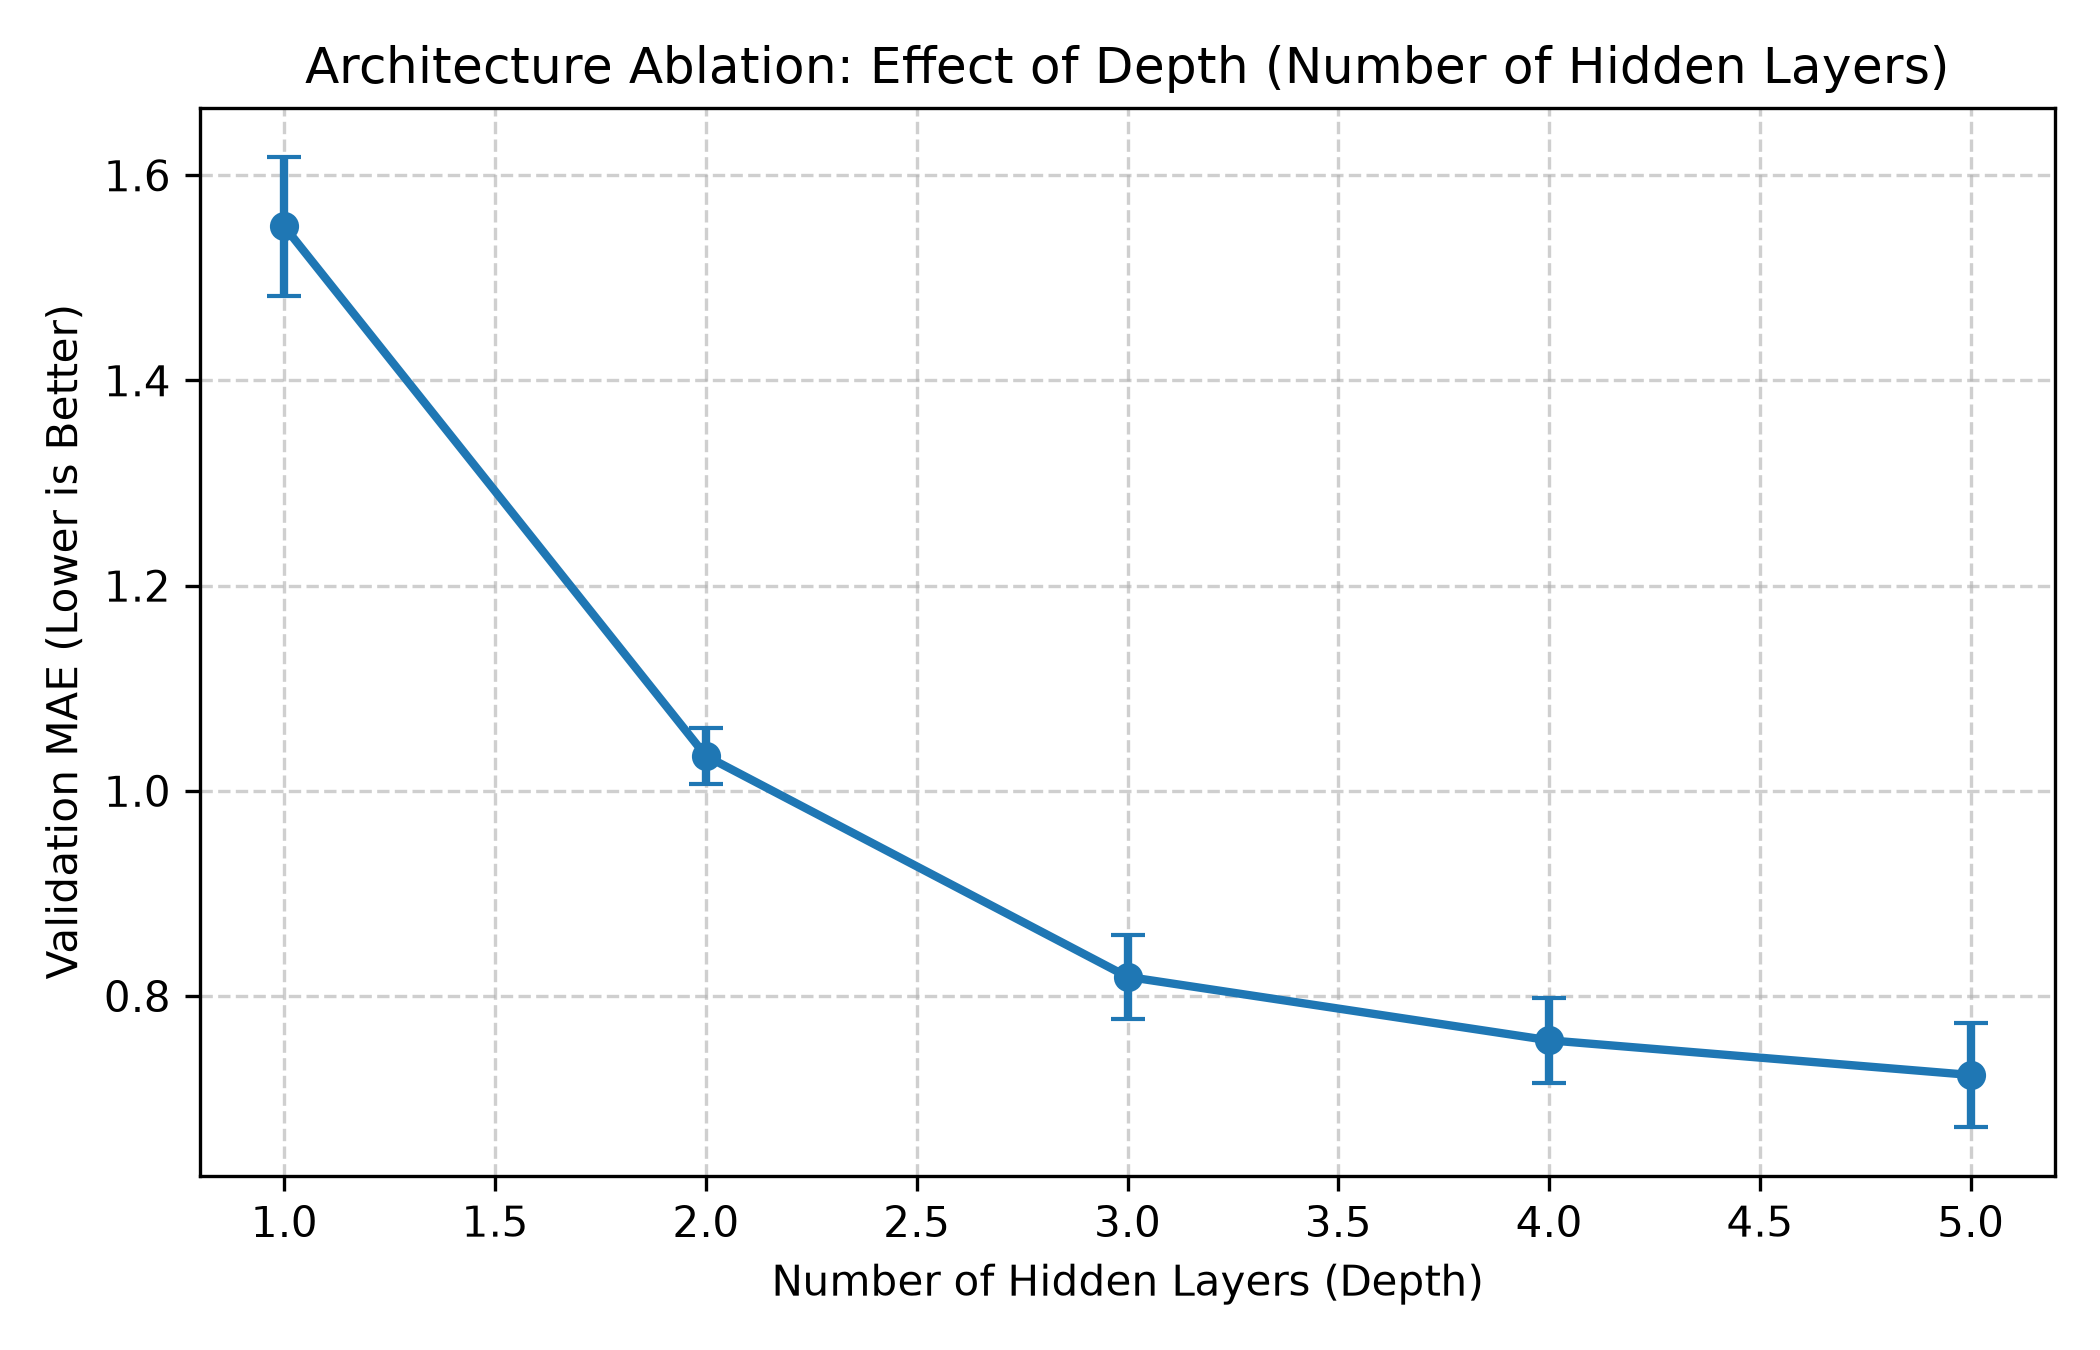
\includegraphics[width=\linewidth]{architecture_depth_sweep.png}
\par\small (a) Depth ablation
\end{minipage}\hfill
\begin{minipage}{0.48\textwidth}
\centering
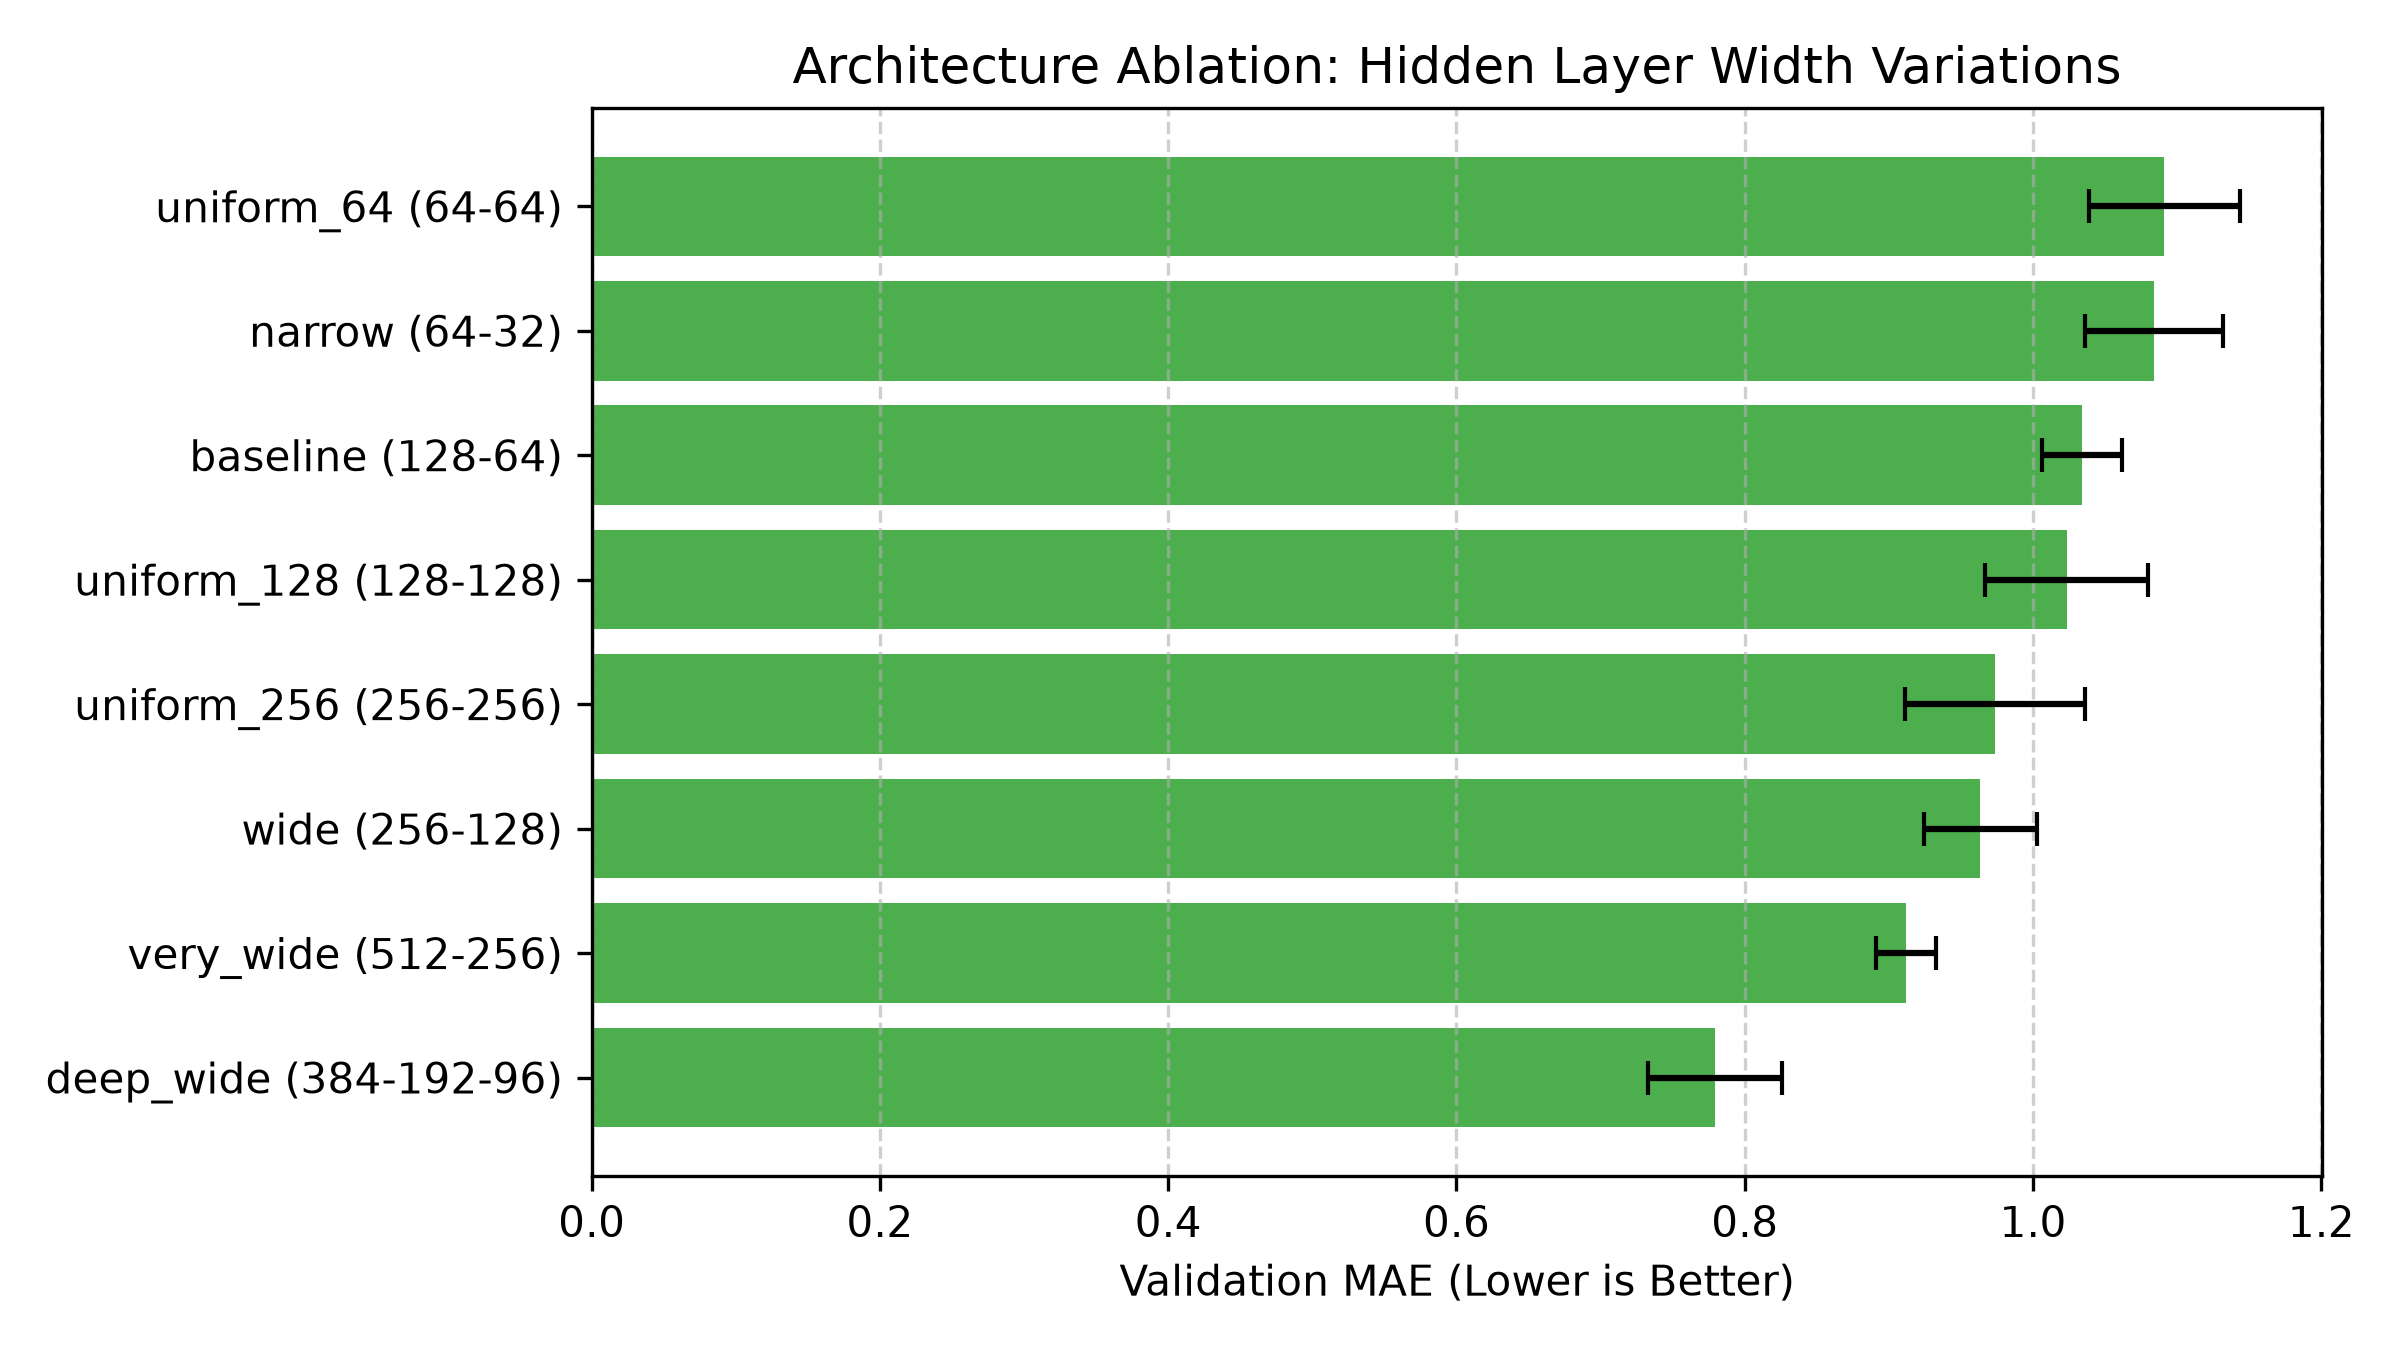
\includegraphics[width=\linewidth]{architecture_width_sweep.png}
\par\small (b) Width ablation
\end{minipage}
\caption{Validation error across the saved MLP architecture sweeps. Lower values indicate better prediction error; corresponding five-seed summaries are reported in Table~\ref{tab:architecture}.}
\label{fig:architecture}
\end{figure*}

Table~\ref{tab:mlpcomparison} comes from the saved comparative result file. It shows that the tuned MLP improves substantially over the base MLP but remains behind the Phase 1 XGBoost on the reported test MAE. This is not a controlled algorithm-only comparison: the MLP uses a 200,000-row training subset, whereas the Phase 1 XGBoost uses the full training partition; the Random Forest also has a different training budget. Test-score standard deviations for the tree models and tuned MLP are not present in this table.

\begin{table}[!t]
\centering
\caption{Saved comparative benchmark across Phase 1 and Phase 2 models. Phase 2 MLPs use a 200,000-row training subset; tree results are inherited from Phase 1 with their original training budgets.}
\label{tab:mlpcomparison}
\resizebox{\linewidth}{!}{%
\begin{tabular}{lrrcc}
\toprule
Model & Parameters & Train rows & Val MAE & Test MAE \\
\midrule
Random Forest & 2,340,000 & 100,000 & 0.4031 & 0.4078 \\
XGBoost & 1,250,000 & 1,986,397 & 0.1040 & 0.0999 \\
Base MLP, ReLU $(128,64)$ & 11,649 & 200,000 & $1.0340\pm0.0277$ & 1.0384 \\
Tuned MLP, GELU $(256,256,256,256)$ & 204,289 & 200,000 & $0.5308\pm0.0465$ & 0.5344 \\
\bottomrule
\end{tabular}}
\end{table}

\subsection{Hybrid ablation}
Table~\ref{tab:hybridablation} uses the five-seed validation CSV from the hybrid notebook. The residual hybrid has lower mean MAE and RMSE than XGBoost alone, and wins on RMSE in all five paired seeds. Its MAE gain is smaller than seed variation. The plain average performs much worse than either XGBoost or the residual hybrid, so a simple average does not explain the residual model's behavior.

\begin{table}[!t]
\centering
\caption{Five-seed hybrid ablation on the validation split (20,000 training rows). Values are mean $\pm$ standard deviation.}
\label{tab:hybridablation}
\resizebox{\linewidth}{!}{%
\begin{tabular}{lccc}
\toprule
Condition & MAE & RMSE & $R^2$ \\
\midrule
XGBoost alone & $0.3988\pm0.1291$ & $0.8573\pm0.1924$ & $0.9978\pm0.0011$ \\
MLP alone & $3.4109\pm0.1629$ & $4.3605\pm0.2021$ & $0.9447\pm0.0052$ \\
Plain 50/50 average & $1.7764\pm0.0897$ & $2.2830\pm0.1101$ & $0.9848\pm0.0015$ \\
Residual hybrid & $0.3888\pm0.1209$ & $0.8027\pm0.1769$ & $0.9981\pm0.0009$ \\
\bottomrule
\end{tabular}}
\end{table}

An earlier results file repeats seed 42 and is not a multi-seed test comparison. A later controlled five-seed test comparison at 20,000 training rows is summarized in Table~\ref{tab:finalcomparison}. Training-row count is controlled, but input feature sets differ, so this is not a feature-matched model-class comparison.

\begin{table*}[!t]
\centering
\caption{Five-seed held-out test comparison at 20,000 training rows. Values are mean $\pm$ standard deviation.}
\label{tab:finalcomparison}
\resizebox{0.98\textwidth}{!}{%
\begin{tabular}{llccc}
\toprule
Model & Feature set & Test MAE & Test RMSE & Test $R^2$ \\
\midrule
XGBoost (Phase 1 tuned) & 23 engineered & $0.2130\pm0.0085$ & $0.5602\pm0.0284$ & $0.9991\pm0.0001$ \\
Residual hybrid & 10 raw & $0.3022\pm0.0499$ & $0.6356\pm0.0824$ & $0.9988\pm0.0003$ \\
XGBoost (hybrid base) & 10 raw & $0.3016\pm0.0501$ & $0.6757\pm0.0949$ & $0.9987\pm0.0004$ \\
Random Forest & 38 features & $0.6545\pm0.0148$ & $1.4543\pm0.0504$ & $0.9939\pm0.0004$ \\
Tuned MLP & 10 raw, quantile normalized & $1.1464\pm0.0537$ & $1.7295\pm0.0721$ & $0.9914\pm0.0007$ \\
Naive mean & Target only & $14.8991\pm0.0159$ & $18.6559\pm0.0012$ & $-0.0006\pm0.0001$ \\
\bottomrule
\end{tabular}}
\end{table*}

In paired seeds, the hybrid has lower RMSE than its raw-feature XGBoost base in all five runs, while its MAE is lower in two of five. Engineered-feature XGBoost outperforms the hybrid in MAE and RMSE in all five paired seeds. These results compare saved configurations, not architecture alone, because their feature sets differ.

The architecture and hybrid notebooks and their raw and aggregate CSVs are included with this report's branch. The former records validation-only Optuna selection and five-seed confirmation; the latter records GroupKFold OOF residual generation and the four-way validation ablation. The companion conference-format PDF contains a different 20,000-row result table; because its figures do not match these saved ablation CSVs, we do not combine or present those values as the same experiment.

\subsection{Leakage checks, geographic errors, and computational cost}
The final comparison audit reports five passed checks: partition row disjointness, train-only transformer fitting, train-only target standardization, zero overlapping areas in GroupKFold, and exclusion of formula-derived or label columns. The controlled comparison uses five seeds and reports held-out test means and standard deviations. Training counts are matched at 20,000, but input feature sets differ. Area and country error summaries are saved; they are descriptive subgroup analyses, not temporal evaluation.

The saved Phase 2 country summary reports XGBoost test MAE of 0.6320 for Canada (584 records), 0.2416 for England, 0.0576 for Ireland, and 0.1157 for the USA. The small Canadian subgroup makes its estimate uncertain. Area-level error summaries are also available, but no time-stratified analysis is saved.

\begin{table}[!t]
\centering
\caption{Measured compute cost and model size at 20,000 training rows on an eight-core ARM system. Inference time is measured per 100,000 rows.}
\label{tab:cost}
\resizebox{\linewidth}{!}{%
\begin{tabular}{lrrrr}
\toprule
Model & Train rows & Parameters / nodes & Train time (s) & Predict / 100k (s) \\
\midrule
Random Forest & 20,000 & 189,884 nodes & 0.387 & 0.1159 \\
XGBoost, engineered & 20,000 & 109,501 nodes & 48.123 & 1.6714 \\
Tuned MLP & 20,000 & 204,289 params & 17.232 & 0.1882 \\
Residual hybrid & 20,000 & 11,777 params (MLP) & 55.260 & 1.8595 \\
\bottomrule
\end{tabular}}
\end{table}
\noindent Timing values describe the saved benchmark hardware and protocol, not universal runtime.

\subsection{Calibration and neural explainability}
For this continuous target, prediction interval coverage probability (PICP) and mean prediction interval width (MPIW) are suitable calibration summaries. The merged project includes Monte Carlo dropout, conformal interval, calibration, and permutation-importance helpers and notebooks, but no executed numerical calibration or feature-importance output is saved. Likewise, the report includes Phase 1 TreeSHAP for XGBoost, but no saved MLP attribution or permutation-importance result. We therefore report neither empirical MLP interval coverage nor MLP feature importance. These are incomplete evaluation items, not positive or negative findings about the methods.

\section{Discussion}
Three findings are supported by the saved Phase 2 results. First, quantile-normal input conditioning improves MLP validation accuracy relative to the Phase 1 preprocessing in the recorded three-seed comparison. Second, the five-seed regularization sweep shows no gain larger than seed variation for this small MLP and 200,000-row training subset; early stopping and the plateau scheduler did not activate within 15 epochs. Third, architecture depth and capacity matter in the recorded ablation, while the separate validation-only Optuna search selects a wider GELU model. These do not imply that one activation or architecture is universally best: the ablation and Optuna outputs describe different model-selection stages.

The hybrid validation ablation is a useful negative-control result: a plain average performs poorly, while the residual hybrid lowers RMSE relative to its raw-feature XGBoost base. The later five-seed test comparison confirms this RMSE pattern but not a consistent MAE advantage. Engineered-feature XGBoost performs best overall in the controlled 20,000-row comparison. The architecture comparison likewise uses fewer training rows for the MLP than for the Phase 1 XGBoost, so it is not an equal-budget model-class test. The Phase 1 leakage interpretation also remains: with the chemical measurements present, models can reconstruct the index formula. A metadata-only regime would be needed to establish broader independent environmental prediction.

\section{Limitations and Outstanding Evaluation}
\label{sec:limitations}
\begin{itemize}
\item The preprocessing result uses three seeds and one MLP configuration; uncertainty across architectures and independent datasets is unknown.
\item The regularization sweep uses 200,000 training rows and a 15-epoch budget. Early stopping and the plateau scheduler did not activate, so their effects remain untested. A full-scale confirmation is needed.
\item Earlier architecture results use 200,000 rows and Phase 1 baselines use larger training partitions. The later controlled comparison uses 20,000 rows for every model, but feature sets differ; this is not a feature-matched comparison.
\item The earlier MLP comparative CSV does not include test standard deviations, while the later controlled five-seed comparison reports test means and standard deviations. Its test comparison uses unequal feature sets, which limits causal interpretation.
\item No executed Phase 2 calibration/interval-coverage result or MLP feature-attribution analysis is available. The calibration helpers alone do not establish calibrated uncertainty.
\item Area- and country-level Phase 2 error summaries and a matched 20,000-row cost table are available. Temporal error analysis remains absent; timing results are specific to the recorded ARM hardware and protocol.
\item Some numerical results in the companion IEEE-format PDF differ from the raw architecture and hybrid CSVs now included with this report. The report uses the CSV-backed values for Phase 2 architecture and hybrid claims and does not combine them with the conflicting summary table.
\item The split estimates performance on unseen monitoring sites, not future years or unseen countries. China has one site and is not represented in the held-out partitions.
\item The CCME target is derived from chemical inputs, so results with those inputs partly measure formula reconstruction. Published upstream imputation and country imbalance further constrain interpretation.
\end{itemize}

\section{Conclusion}
Phase 1 established the data-cleaning and split pipeline, baselines, tree ensembles, and the key finding that full-measurement accuracy largely reconstructs the CCME formula; withholding measurements causes substantial performance loss. Phase 2 reused the leakage controls and extended the comparison with MLP input conditioning, architecture and regularization ablations, and a GroupKFold residual hybrid. Quantile-normal preprocessing improved the recorded MLP validation result; the regularization sweep found no gain beyond seed variation; the architecture study selected a tuned MLP that improved on the base MLP but remained behind the full-data XGBoost result under unequal training budgets. In the five-seed hybrid validation ablation, residual learning beat the plain average; a later five-seed test comparison confirmed lower RMSE than the raw-feature XGBoost base but not a consistent MAE gain. Engineered-feature XGBoost achieved the strongest overall results in the controlled comparison. Empirical calibration and MLP feature-attribution results, and a temporal error breakdown, remain unreported; those gaps prevent a claim that every planned Phase 2 evaluation was completed.

\bibliographystyle{IEEEtran}
\bibliography{../../docs/refs_dl,../../docs/refs}
\end{document}
